\let\negmpace\undefined
\let\negthickspace\undefined
\documentclass[journal]{IEEEtran}
\usepackage[a5paper, margin=10mm, onecolumn]{geometry}
%\usepackage{lmodern} % Ensure lmodern is loaded for pdflatex
\usepackage{tfrupee} % Include tfrupee package
\setlength{\headheight}{1cm} % Set the height of the header box
\setlength{\headsep}{0mm}     % Set the distance between the header box and the top of the text
\usepackage{gvv-book}
\usepackage{gvv}
\usepackage{cite}
\usepackage{amsmath,amssymb,amsfonts,amsthm}
\usepackage{algorithmic}
\usepackage{graphicx}
\usepackage{textcomp}
\usepackage{xcolor}
\usepackage{txfonts}
\usepackage{listings}
\usepackage{enumitem}
\usepackage{mathtools}
\usepackage{gensymb}
\usepackage{comment}
\usepackage[breaklinks=true]{hyperref}
\usepackage{tkz-euclide} 
\usepackage{listings}
% \usepackage{gvv}                                        
\def\inputGnumericTable{}                                 
\usepackage[latin1]{inputenc}                                
\usepackage{color}                                            
\usepackage{array}                                            
\usepackage{longtable}                                       
\usepackage{calc}                                             
\usepackage{multirow}                                         
\usepackage{hhline}                                           
\usepackage{ifthen}                                           
\usepackage{lscape}
\renewcommand{\thefigure}{\theenumi}
\renewcommand{\thetable}{\theenumi}
\setlength{\intextsep}{10pt} % Space between text and floats
\numberwithin{equation}{enumi}
\numberwithin{figure}{enumi}
\renewcommand{\thetable}{\theenumi}
\begin{document}
\bibliographystyle{IEEEtran}
\title{Question-1-1.5-2}
\author{EE24BTECH11035 - KOTHAPALLI AKHIL}
% \maketitle
% \newpage
% \bigskip
{\let\newpage\relax\maketitle}
\textbf{Question}:\\
Find the ratio in which the Y axis divides divides the line segment joining points $(6,-4)$ and $(-2,-7)$.Also find the point of intersection.\\
\textbf{Solution}:\\
\begin{table}[h!]
   \centering
	\begin{tabular}{|c|c|c|}
\hline
\textbf{Line Equation} & \textbf{h value} & \textbf{m}\\
\hline
$3x - 2y + 1 = 0$ & $\left( \begin{array}{c} 3 \\ -2 \end{array} \right)$ & 1 \\
\hline
$2x + 3y - 21 = 0$ & $\left( \begin{array}{c} 2 \\ 3 \end{array} \right)$ & -21 \\
\hline
$x - 5y + 9 = 0$ & $\left( \begin{array}{c} 1 \\ -5 \end{array} \right)$ & 9 \\
\hline
\end{tabular}



   \caption{variables used}
   \label{tabQuestion-1-1.5-17}
\end{table}   

Let the point on the Y-axis be $\myvec{0\\y}$, \\ The given two points are \myvec{6\\-4} and \myvec{-2\\-7}.  \\
The above 3 points are collinear.\\\\
Construct a Matrix for the above points
\begin{align}
   M= \myvec{0 & y & 1\\6 & -4 & 1\\-2 &-7 & 1}
\end{align}
The Determinant of the matrix is 0
\begin{align}
   Det=0(-4+7)-y(6+2)+1(-42-8)=0\\
    \implies y=-6.25
\end{align}\\
$\therefore$ The point on Y-Axis is \myvec{0\\-6.25}


Assume point $\vec{B}$ divides the line segment $\vec{AC}$ in the ratio  k:1.  According to the section formula:
\begin{equation}
\vec{B} = \frac{k\vec{C}+\vec{A}}{k+1}
\end{equation}
Substituting the values:
\begin{equation}
\myvec{0 \\ -6.25}  = \frac{k \myvec{-2 \\ -7} +  \myvec{6 \\ -4} }{k+1}
\end{equation}
This gives us two equations:
\begin{equation}
0 = \frac{-2k + 6}{k+1}, \quad -6.25 = \frac{-7k - 4}{k+1}
\end{equation}
Solving for k from the first equation:
\begin{equation}
0 = -2k + 6 \\
\Rightarrow  2k = 6 \\
\Rightarrow k = 3 \\
\end{equation}
Therefore, the ratio in which  $\vec{B}$  divides $\vec{AC}$ is  3:1 .
\begin{figure}[h!]
	\centering
	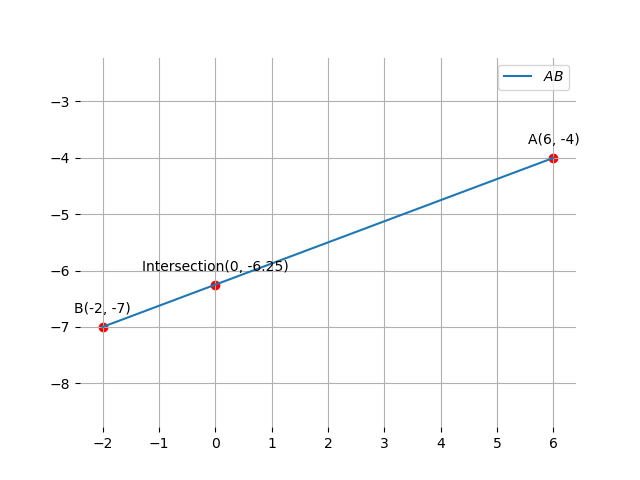
\includegraphics[width=0.5\linewidth]{figs/Figure_1.png}
	\caption{ Line $\vec{A}\vec{C}$}
	\label{stemplot}
\end{figure}	

\end{document}
